\chapter{Arhitektura i dizajn sustava}
		
		\textbf{\textit{dio 1. revizije}}\\

		Arhitektura naše aplikacije, može se podijeliti na sljedeće komponente
	\begin{itemize}
		\item 	Server strana (\textit{backend})
		\item 	Klijent strana (\textit{frontend})
		\item 	Baza podataka (\textit{db})		
	\end{itemize}
	\textbf{Server strana} je glavna komponenta naše aplikacije. U njoj se nalazi programska logika koja se brine da korisnik može dohvatiti sve podatke koji mu trebaju ili spremiti iste. Komunikaciju prema klijentskoj strani smo ostvarili korištenjem GraphQL-om. \\
	\textbf{Baza podataka} koju smo koristili je PostgreSQL. Kako bi izbjegli programske greške u SQLu te potencijalne ranjivosti (Npr SQL Injekcija), za komunikaciju s bazom koristili smo ORM (Object Relation Mapper) \textit{TypeORM}. Kroz \textit{TypeORM} dobili smo i sustav za verzioniranje baza podataka "migracije", tako da možemo lakše i sigurnije raditi izmjene na bazi, te dijeliti te izmjene između programera u timu i produkcijskih servera. \\
	\textbf{Klijentska strana} je grafičko sučelje s kojim krajnji korisnik pristupa aplikaciji. U našem slučaju implementirano je kao SPA (Single Page Application) sa \textit{React}-om. \\
	
	\begin{figure}[H]
		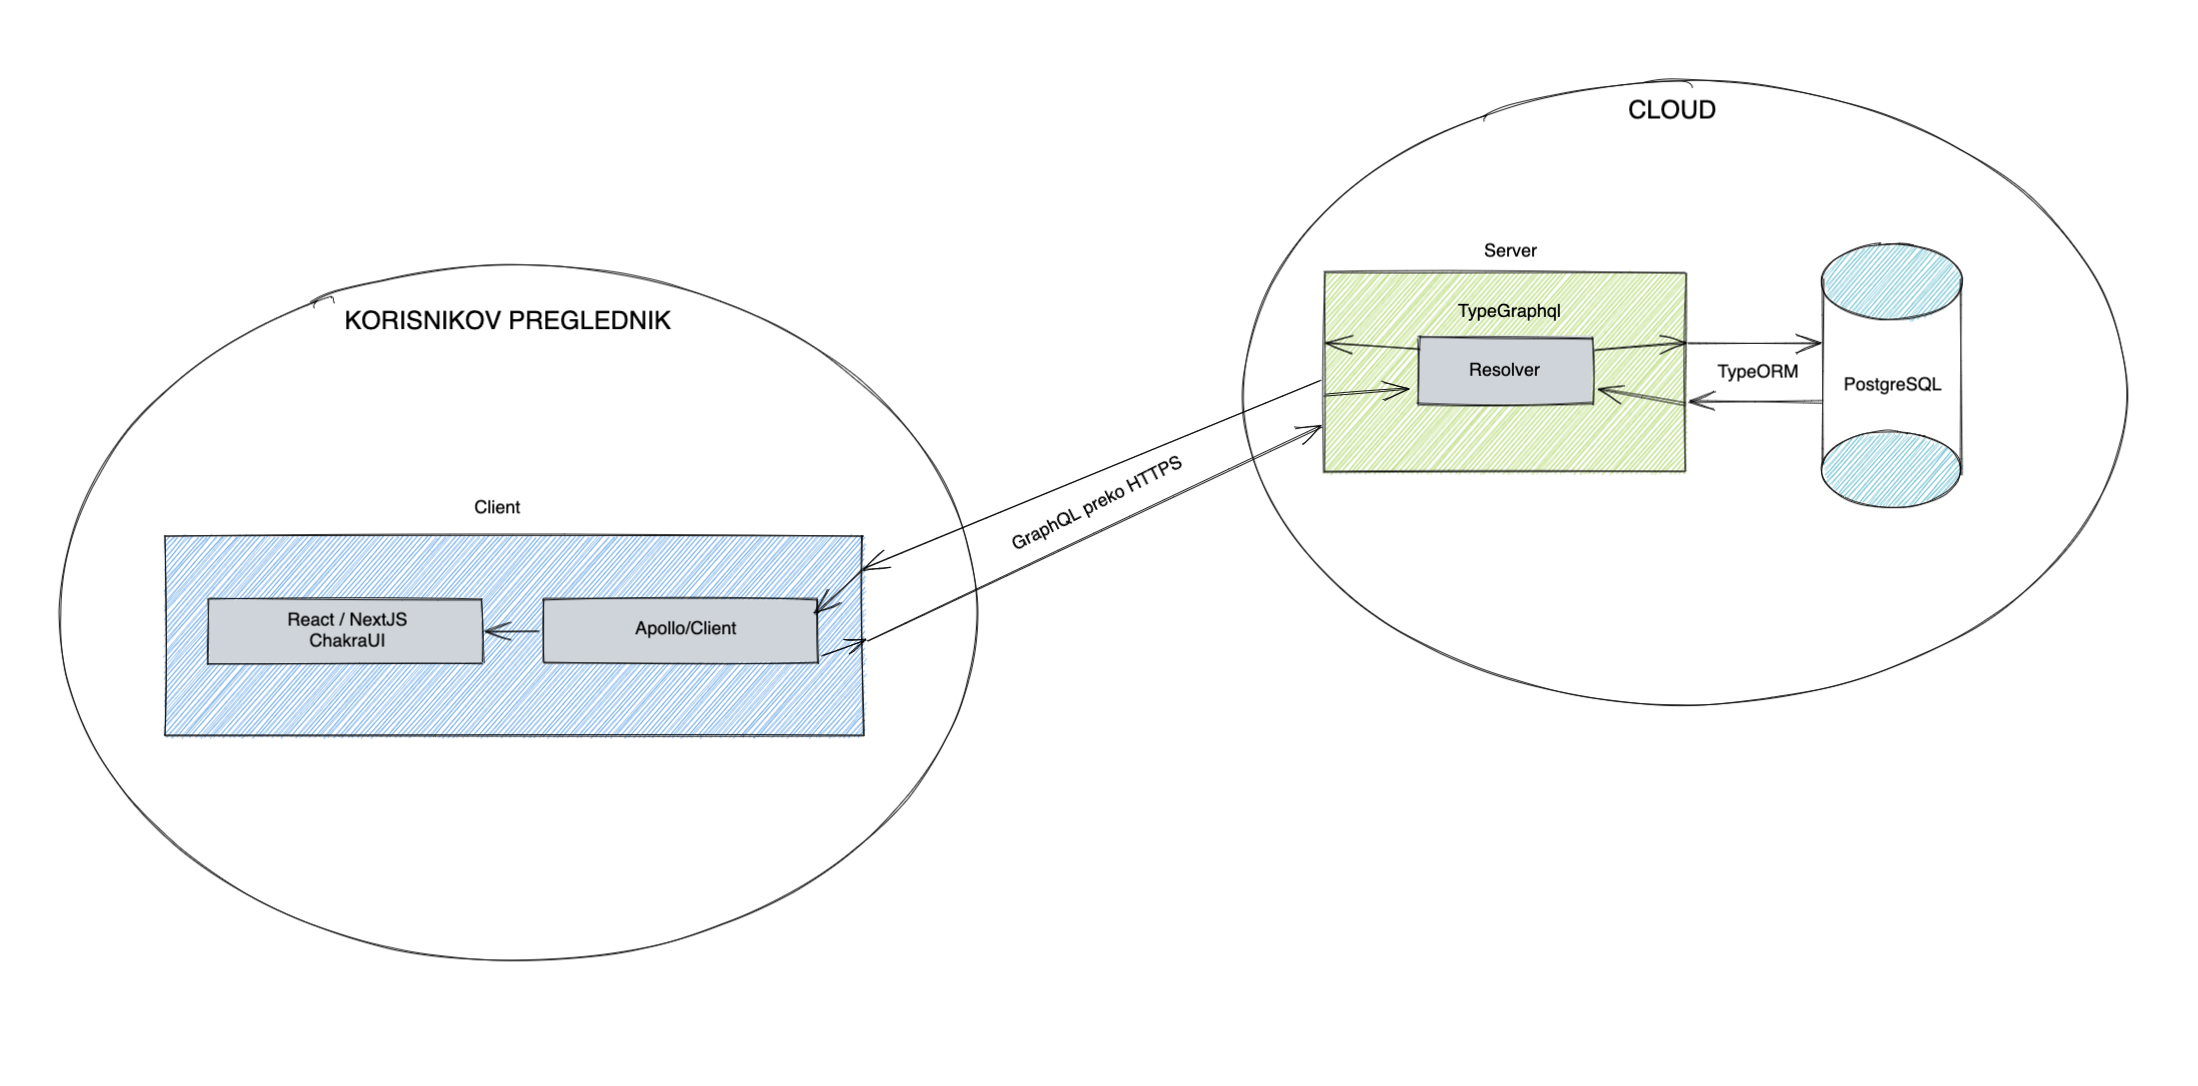
\includegraphics[width=\textwidth]{slike/arhitekturaDijagram.png} 
		\caption{Model arhitekture}
		\label{fig:arhitektura} 
	\end{figure}

				
		\section{Baza podataka}
			
			\textbf{\textit{dio 1. revizije}}\\
			
		U našem sustavu korisimo PostgreSQL relacijsku bazu podataka za spremanje informacija o potresima i upitnicima.
		U bazi podataka imamo sljedeće entitete:
		\begin{itemize}
			\item 	users
			\item 	earthquakes
			\item 	surveys
		\end{itemize}

			\subsection{Opis tablica}
			
				Tablica u kojoj se spremaju pristupni podaci te uloge korisnika u sustavu.
				\begin{longtblr}[
					label=none,
					entry=none
					]{
						width = \textwidth,
						colspec={|X[7,l]|X[7, l]|X[20, l]|}, 
						rowhead = 1,
					} %definicija širine tablice, širine stupaca, poravnanje i broja redaka naslova tablice
					\hline \multicolumn{3}{|c|}{\textbf{users}}	 \\ \hline[3pt]
					\SetCell{LightGreen}id & INT	&  	id korisnika  	\\ \hline
					created\_at	& TIMESTAMP &  vremenski žig kada je korisnik stvoren	\\ \hline 
					updated\_at	& TIMESTAMP &  vremenski žig kada je korisnik izmijenjen 	\\ \hline 
					email & VARCHAR &  email adresa korisnika \\ \hline 
					password\_hash & VARCHAR &  lozinka korisnika spremljena kao hash \\ \hline 
					role & Enum:UserRole &  uloga korisnika (admin i seizmolog) \\ \hline 
				\end{longtblr}

				Tablica u kojoj se spremaju prošli potresi, svaki potres može imati 0:n upitnika koje su građani ispunili.
				\begin{longtblr}[
					label=none,
					entry=none
					]{
						width = \textwidth,
						colspec={|X[7,l]|X[7, l]|X[20, l]|}, 
						rowhead = 1,
					} %definicija širine tablice, širine stupaca, poravnanje i broja redaka naslova tablice
					\hline \multicolumn{3}{|c|}{\textbf{earthquakes}}	 \\ \hline[3pt]
					\SetCell{LightGreen}id & INT	&  	id potresa  	\\ \hline
					created\_at	& TIMESTAMP &  vremenski žig kada je potres stvoren	\\ \hline 
					updated\_at	& TIMESTAMP &  vremenski žig kada je potres izmijenjen 	\\ \hline 
					name & VARCHAR &  naziv potresa \\ \hline 
					strength & REAL &  jačina potresa \\ \hline 
					epicenter\_lat & REAL &  geografska širina epicentra \\ \hline 
					epicenter\_lng & REAL &  geografska dužina epicentra \\ \hline 
					date	& TIMESTAMP &  vremenski žig kada se potres dogodio 	\\ \hline 
				\end{longtblr}

				Tablica u kojoj se nalaze ispunjeni upitnici.
				\begin{longtblr}[
					label=none,
					entry=none
					]{
						width = \textwidth,
						colspec={|X[7,l]|X[7, l]|X[20, l]|}, 
						rowhead = 1,
					} %definicija širine tablice, širine stupaca, poravnanje i broja redaka naslova tablice
					\hline \multicolumn{3}{|c|}{\textbf{surveys}}	 \\ \hline[3pt]
					\SetCell{LightGreen}id & INT	&  	id upitnika  	\\ \hline
					created\_at	& TIMESTAMP &  vremenski žig kada je upitnik stvoren	\\ \hline 
					updated\_at	& TIMESTAMP &  vremenski žig kada je upitnik izmijenjen 	\\ \hline 
					lat & REAL &  geografska širina upitnika \\ \hline 
					lng & REAL &  geografska dužina upitnika \\ \hline 
					\SetCell{LightBlue}earthquakeId	& INT &  id potresa za koji je ovaj upitnik ispunjen 	\\ \hline 
				\end{longtblr}

			
			\subsection{Dijagram baze podataka}

				\begin{figure}[H]
					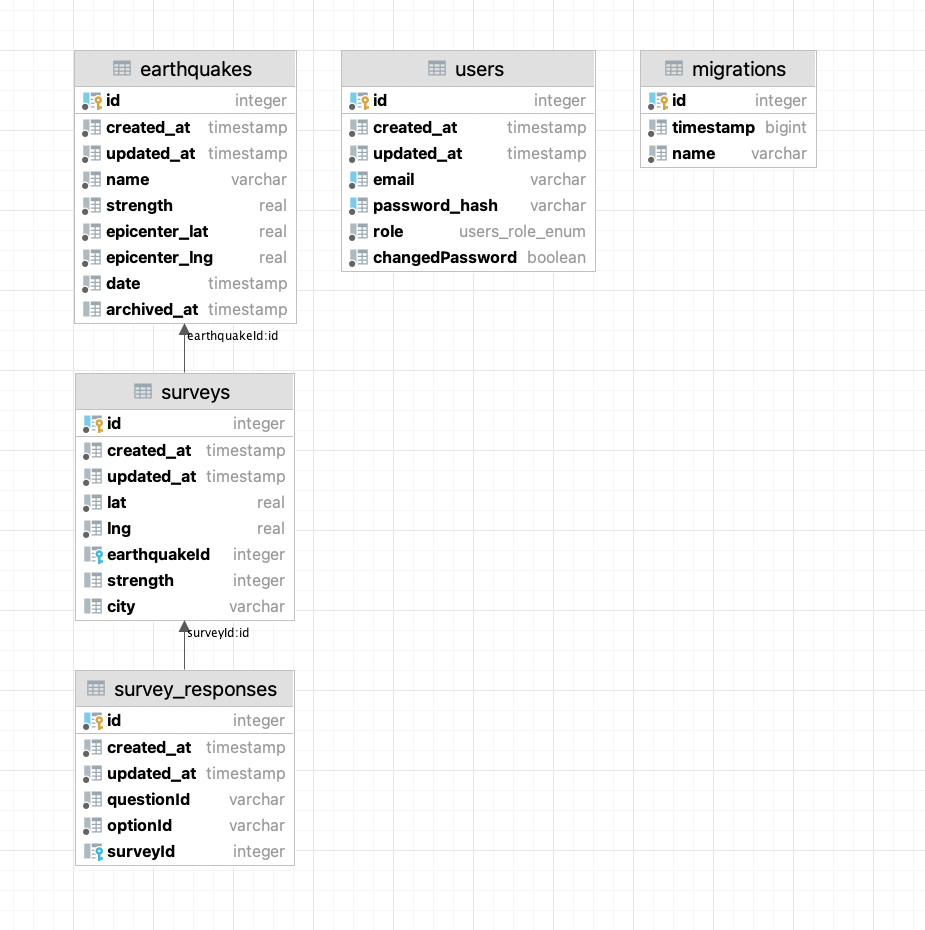
\includegraphics[width=\textwidth]{slike/tectonicDBDiagram.png} 
					\caption{Dijagram baze podataka}
					\label{fig:baza} 
				\end{figure}

			\eject
			
			
		\section{Dijagram razreda}
			
			\begin{figure}[H]
				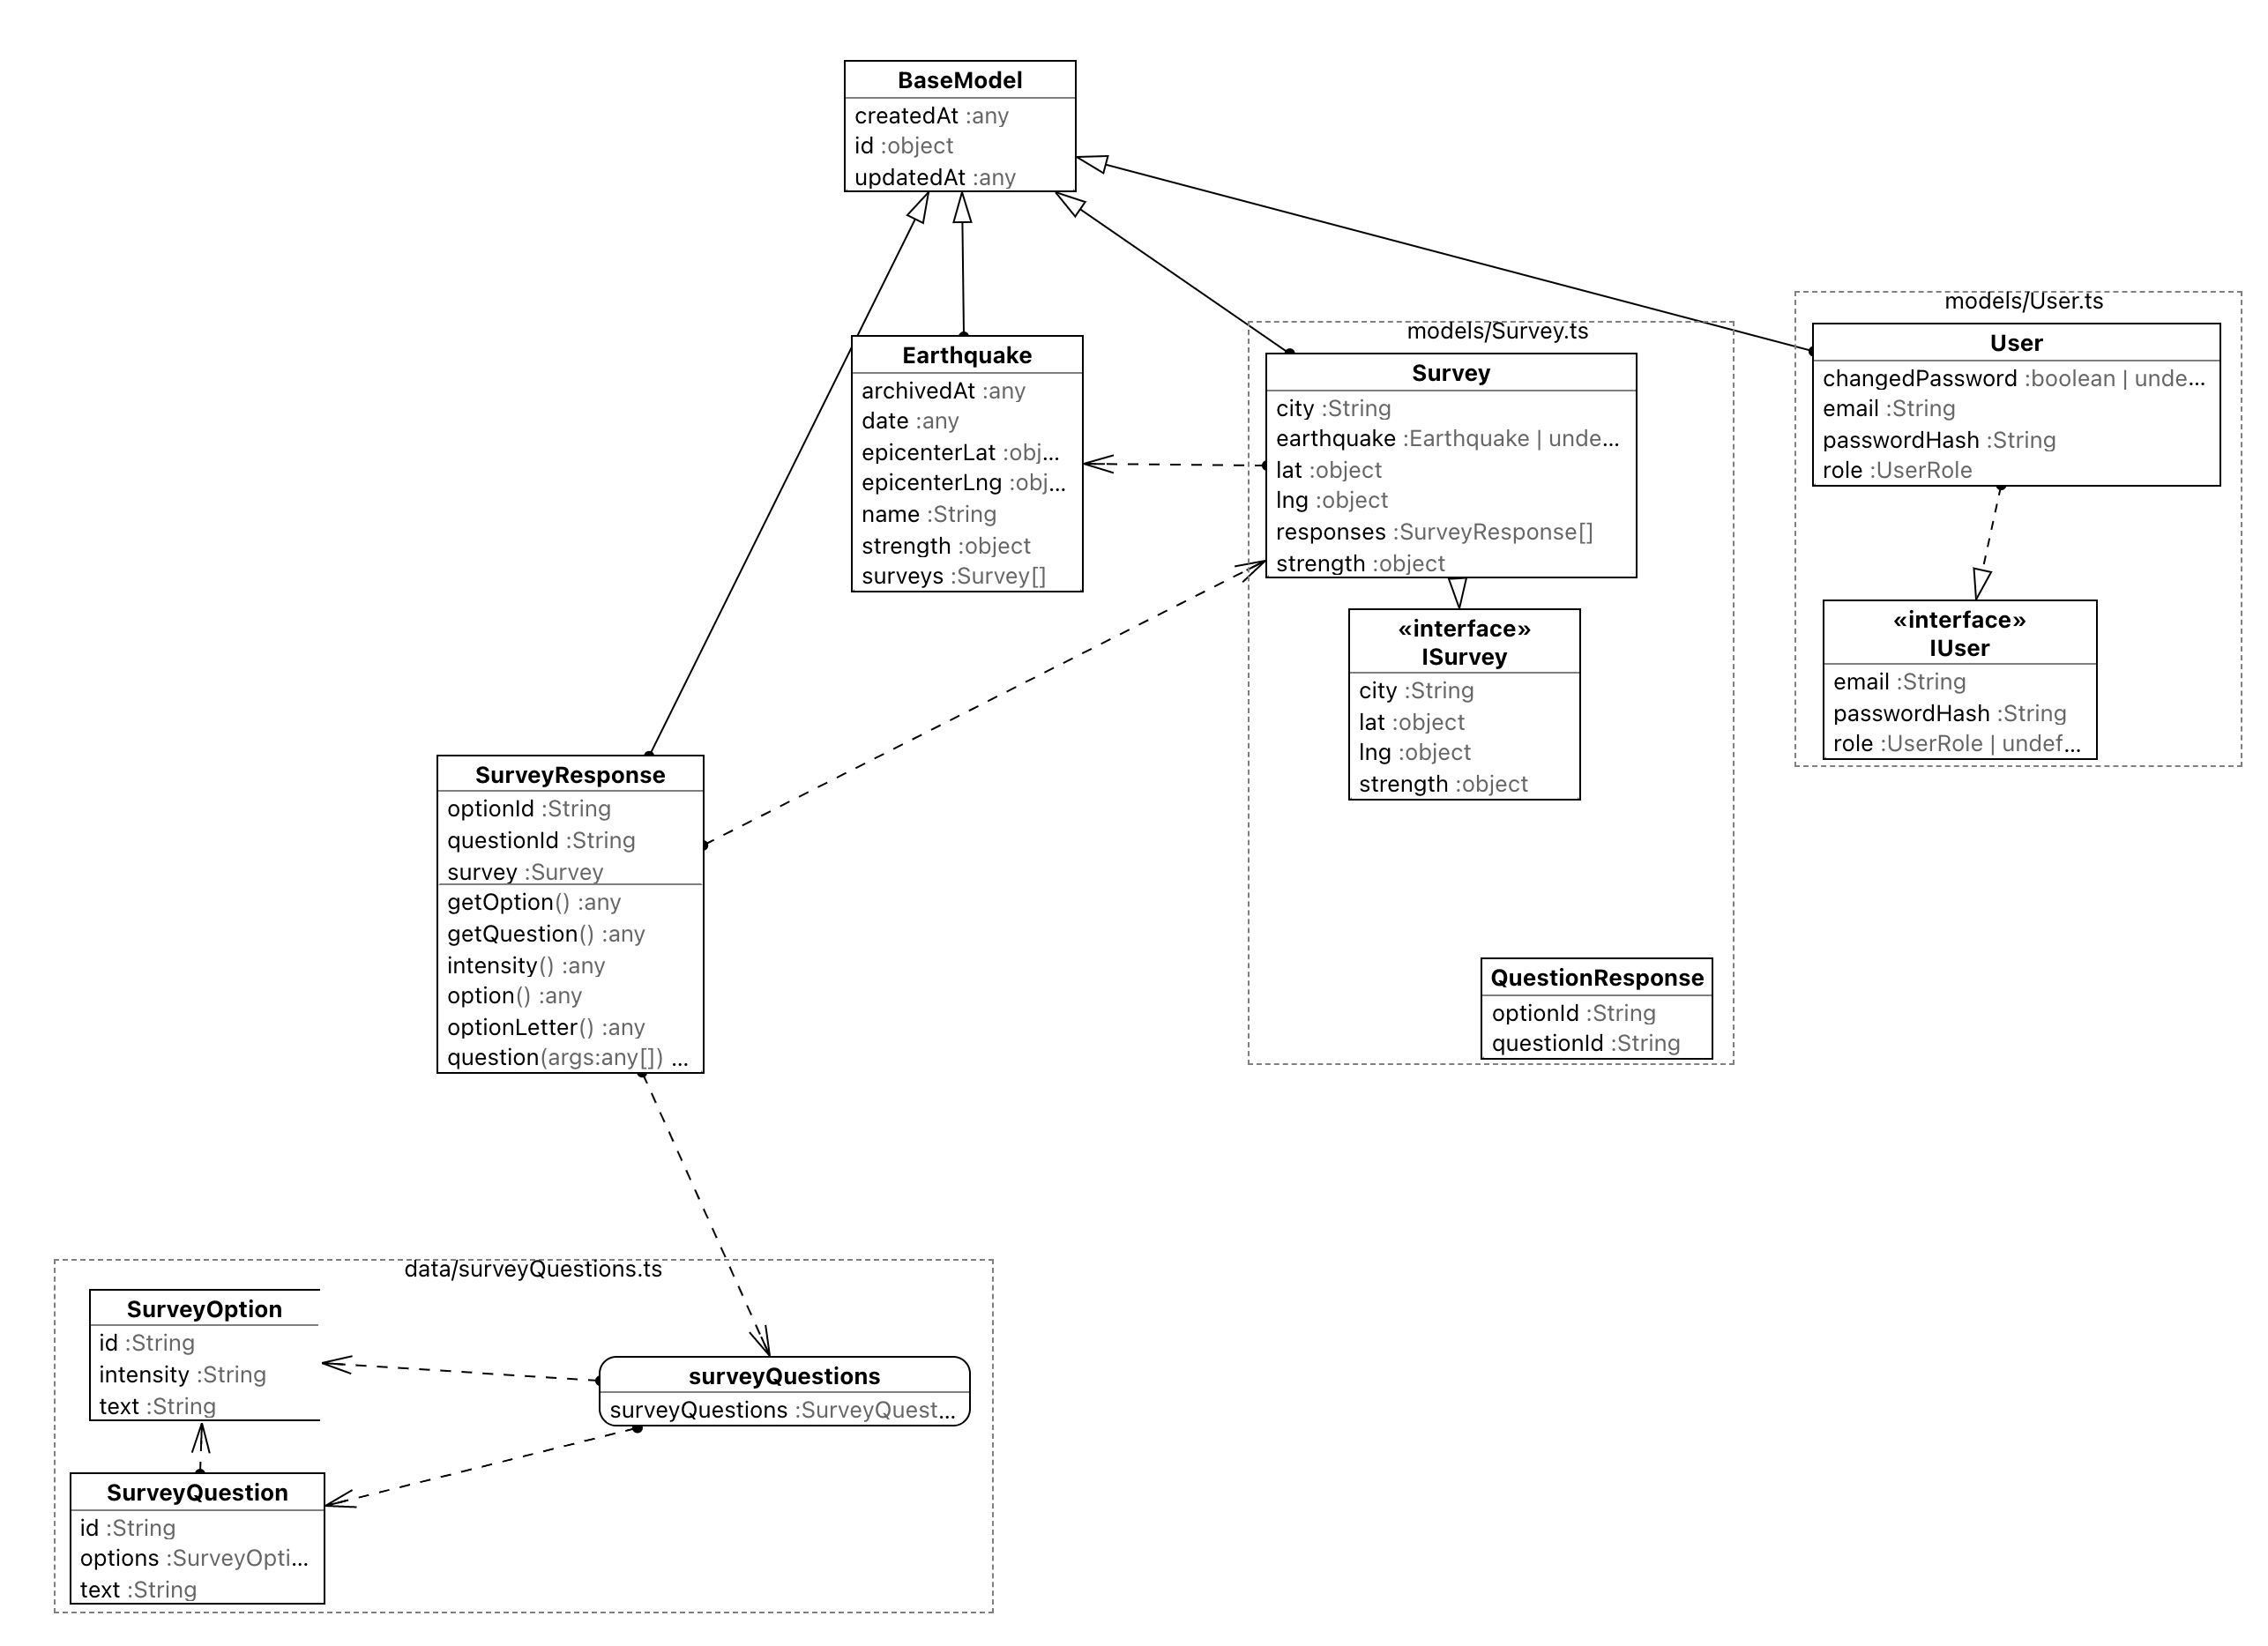
\includegraphics[width=\textwidth]{slike/classdiagram_only_db.png} 
				\caption{Dijagram razreda za modeliranje baze podataka}
				\label{fig:uml_db} 
			\end{figure}

			\begin{figure}[H]
				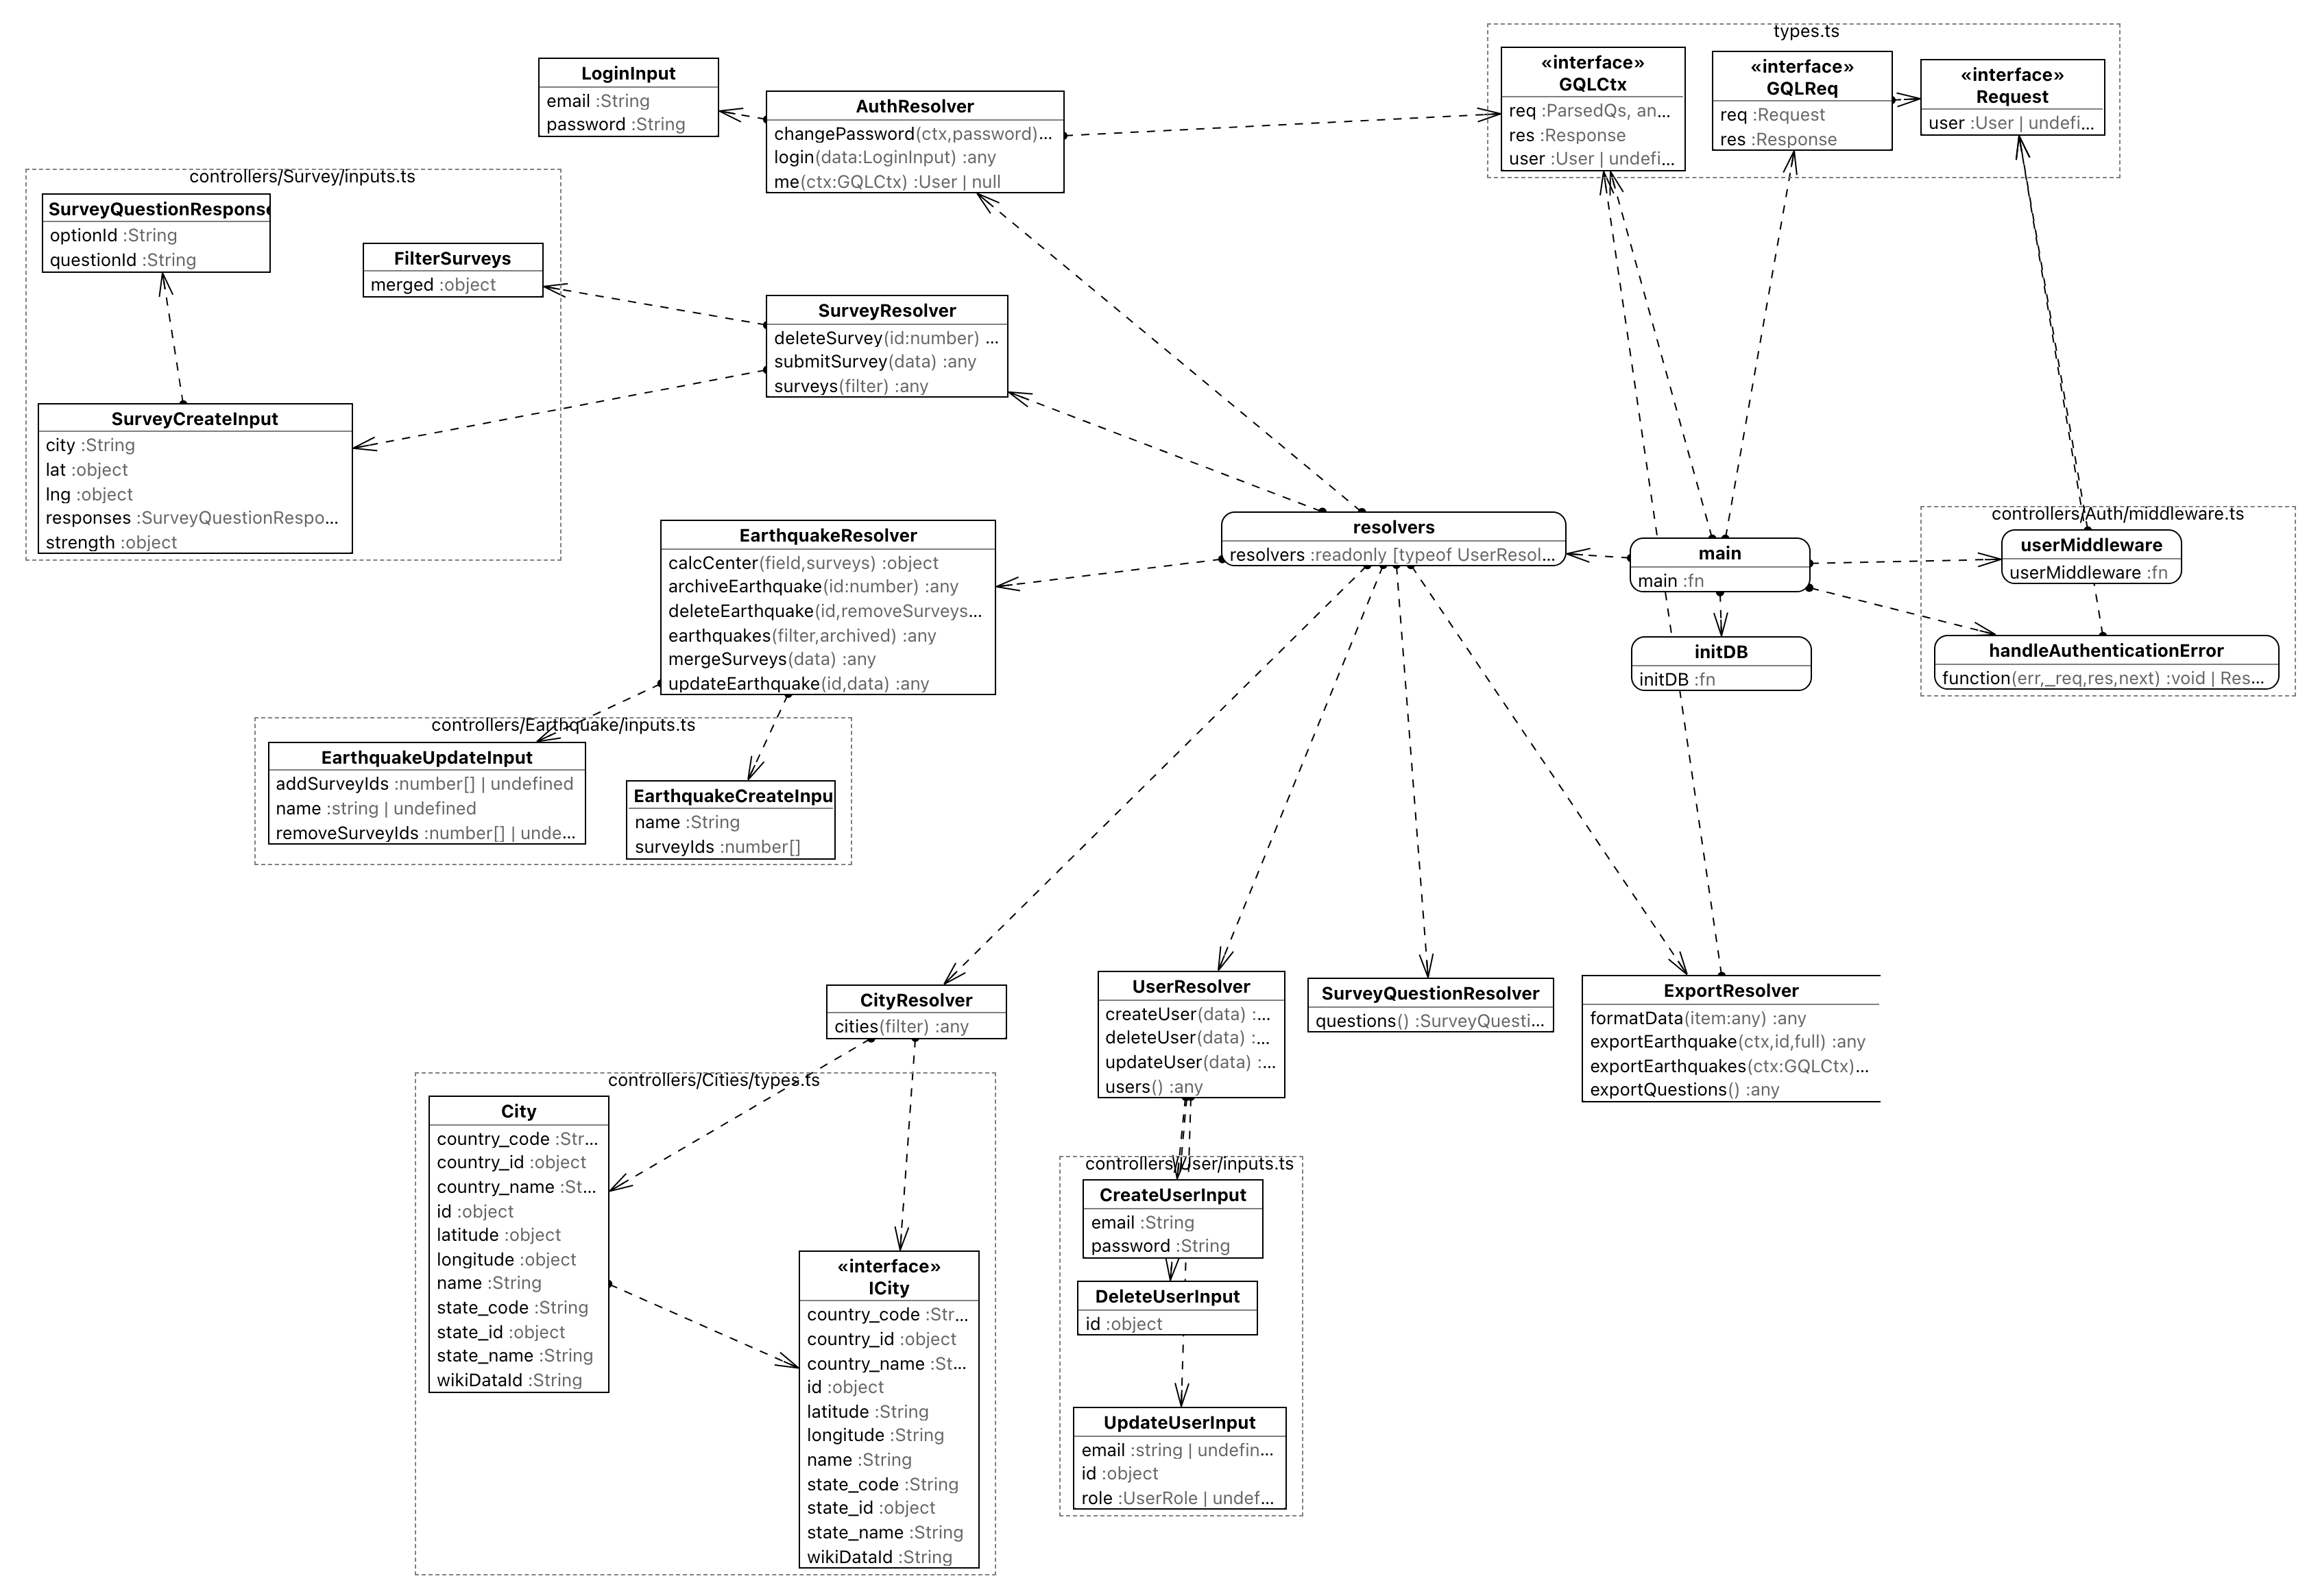
\includegraphics[width=\textwidth]{slike/classdiagram_no_db.png} 
				\caption{Dijagram razreda bez baze podataka}
				\label{fig:uml_no_db} 
			\end{figure}

			\begin{figure}[H]
				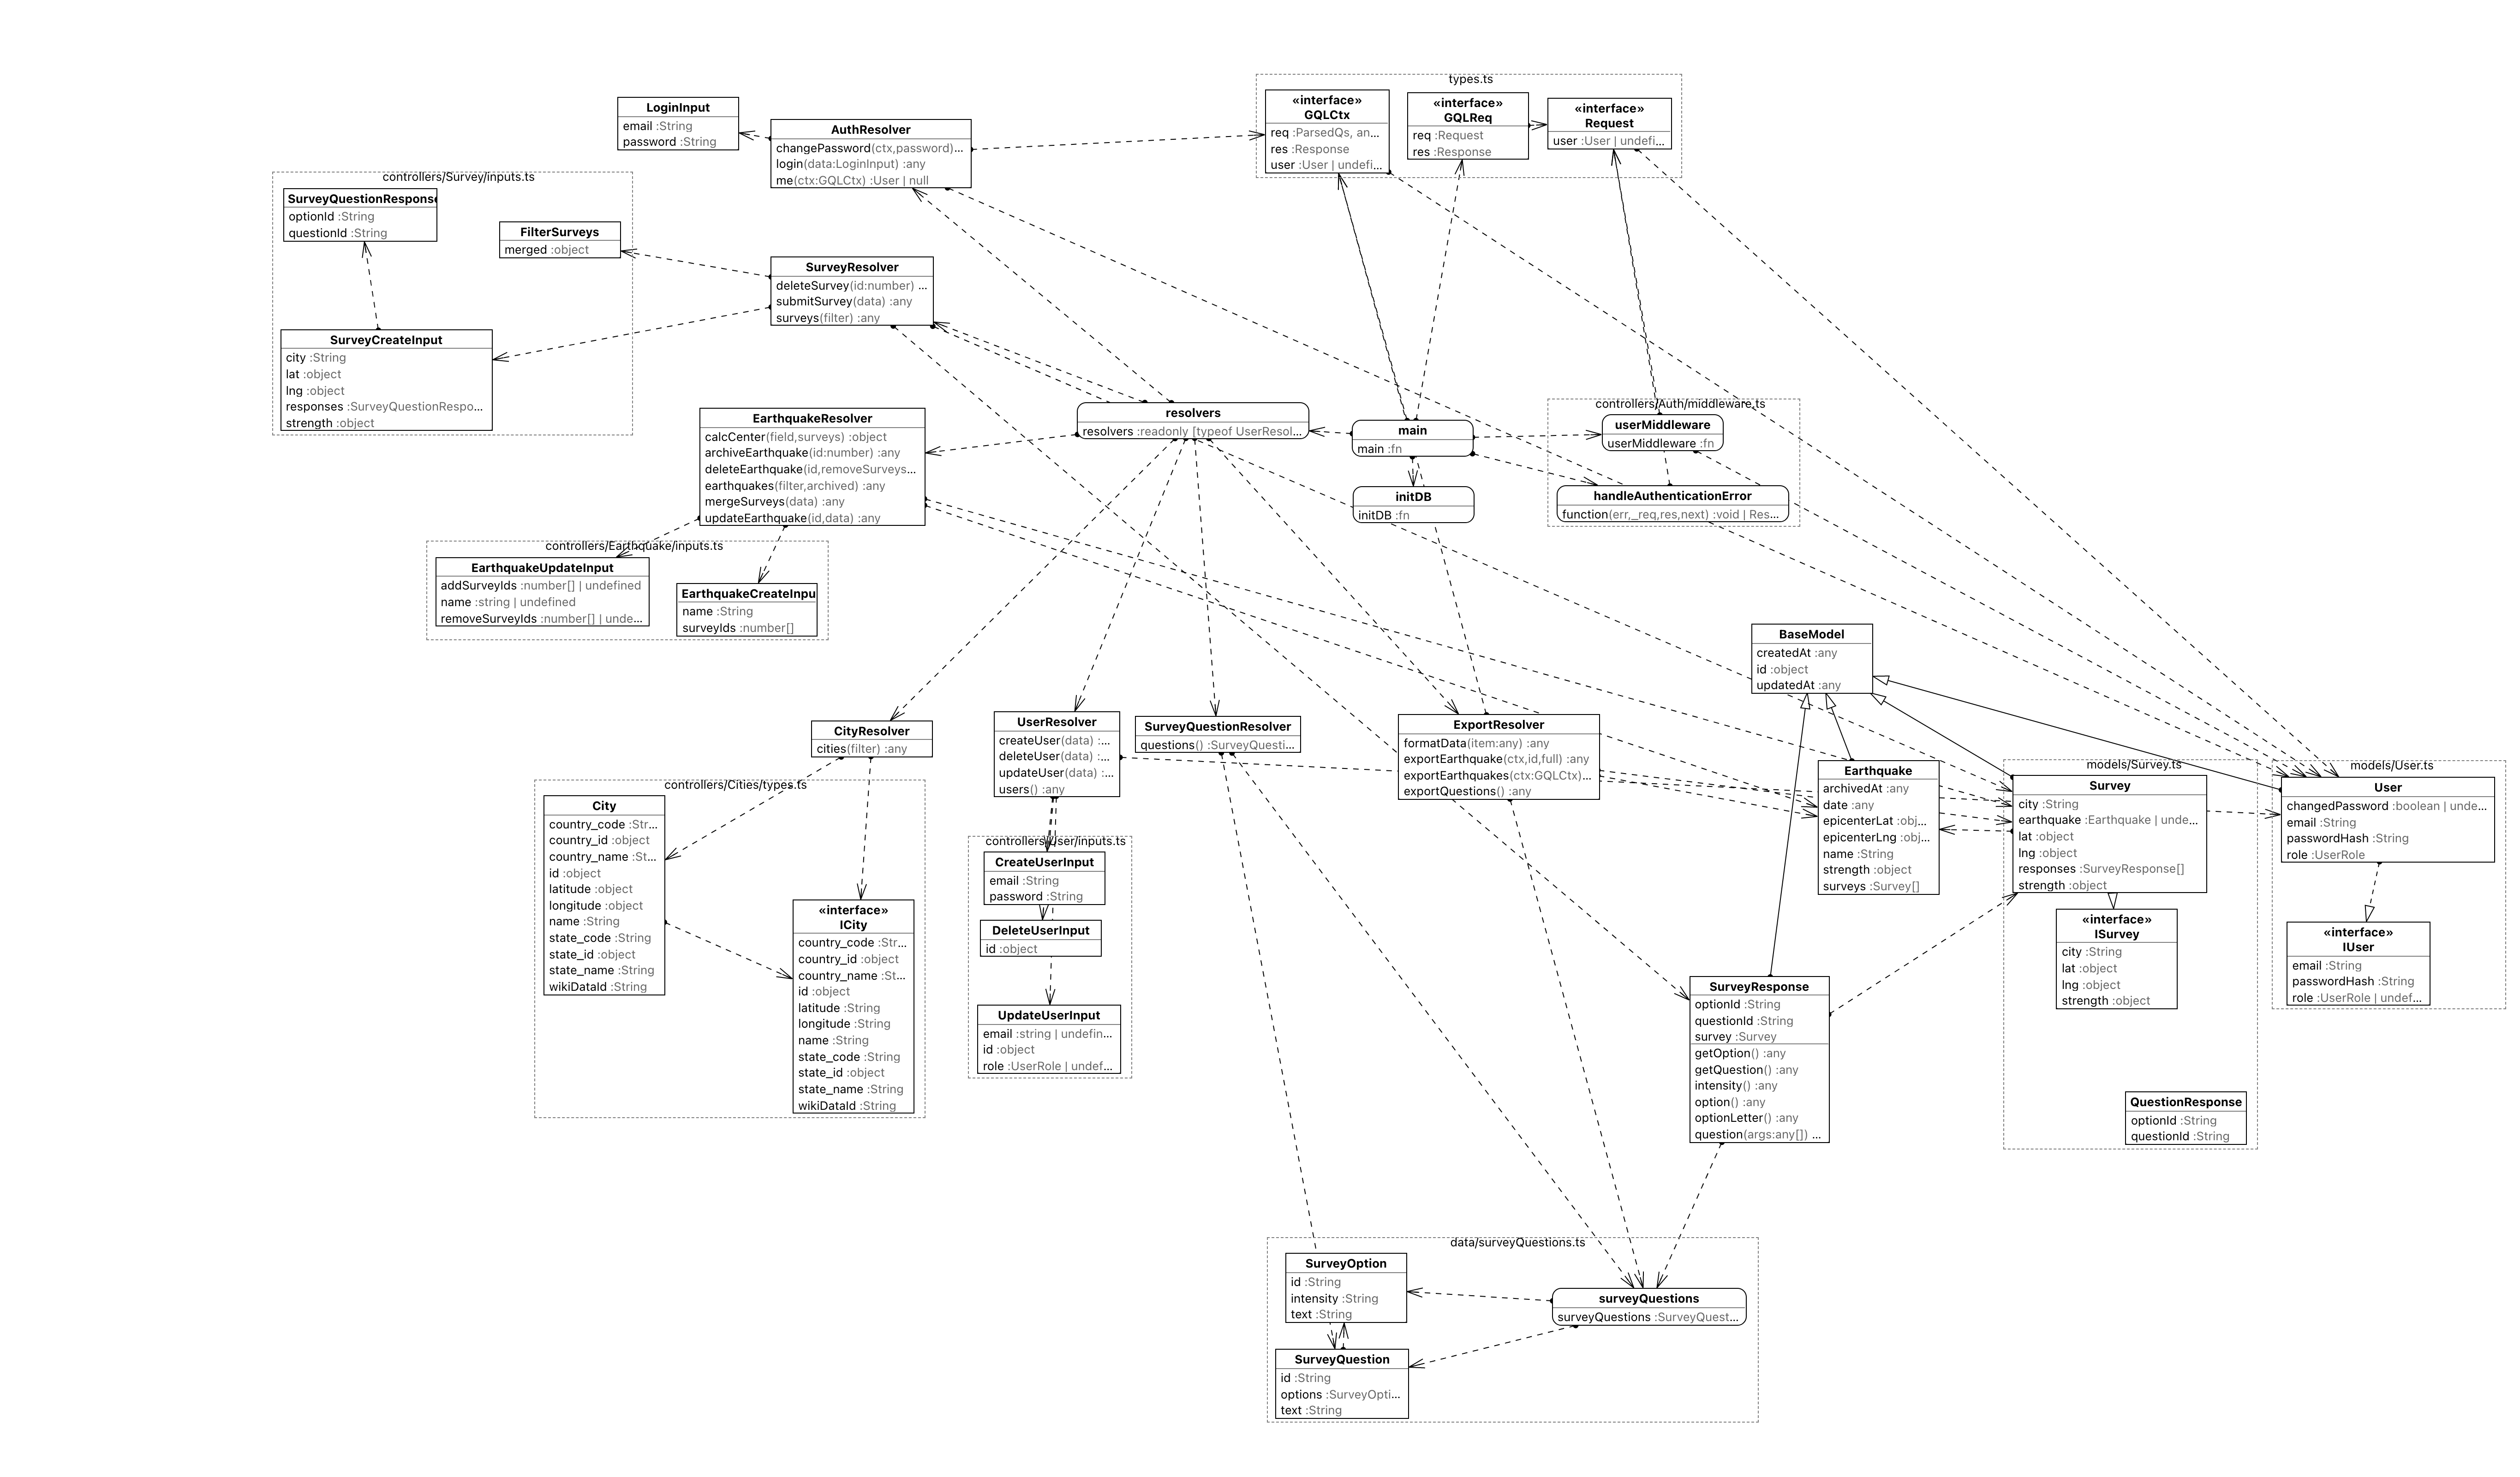
\includegraphics[width=\textwidth]{slike/classDiagram.png} 
				\caption{Dijagram razreda cijele aplikacije}
				\label{fig:uml} 
			\end{figure}

			\textbf{\textit{dio 2. revizije}}\\			
			
			\textit{Prilikom druge predaje projekta dijagram razreda i opisi moraju odgovarati stvarnom stanju implementacije}
			
			
			
			
			\eject
		
		\section{Dijagram stanja}
			
			
			\textbf{\textit{dio 2. revizije}}\\
			
			\textit{Potrebno je priložiti dijagram stanja i opisati ga. Dovoljan je jedan dijagram stanja koji prikazuje \textbf{značajan dio funkcionalnosti} sustava. Na primjer, stanja korisničkog sučelja i tijek korištenja neke ključne funkcionalnosti jesu značajan dio sustava, a registracija i prijava nisu. }
			
			
			\eject 
		
		\section{Dijagram aktivnosti}
			
			\textbf{\textit{dio 2. revizije}}\\
			
			 \textit{Potrebno je priložiti dijagram aktivnosti s pripadajućim opisom. Dijagram aktivnosti treba prikazivati značajan dio sustava.}
			
			\eject
		\section{Dijagram komponenti}
		
			\textbf{\textit{dio 2. revizije}}\\
		
			 \textit{Potrebno je priložiti dijagram komponenti s pripadajućim opisom. Dijagram komponenti treba prikazivati strukturu cijele aplikacije.}